\chapter{असममित संश्लेषण}\label{ch:b3:asymmetric-synthesis}

L-डोपा, वह औषध जो पार्किंसन रोग के लक्षणों को कम करती है,
1970 के दशक में \omterm{def:b3:asymmetric-synthesis:asymmetric-catalysis}{असममित उत्प्रेरण} द्वारा औद्योगिक रूप से बना पहला यौगिक था: एक समतल, अकिरैल पूर्वगामी के साथ
हाइड्रोजन के अधीन घुले एक किरैल रोडियम संकुल के कुछ ग्रामों ने ऐसा उत्पाद दिया जिसमें एक प्रतिबिंबरूपी
दूसरे से कहीं अधिक था। किसी औषध के दोनों प्रतिबिंबरूपियों के प्रभाव पूरी तरह भिन्न हो सकते हैं,
क्योंकि जिन ग्राहियों और \omterm{def:b3:complex-kinetics:enzyme}{एंज़ाइमों} से वे मिलते हैं वे स्वयं किरैल हैं। यह
अध्याय प्रतिबिंबरूपी शुद्धता को मापता है, समझाता है कि एक किरैल परिवेश दो दर्पण-प्रतिबिंब पथों के बीच
कैसे चुनता है, और उन रणनीतियों (\omterm{def:b3:asymmetric-synthesis:chiral-pool}{किरैल कुंड},
सहायक, विभेदन, धात्विक और कार्बनिक उत्प्रेरक) से गुज़रता है जो एकल
प्रतिबिंबरूपी बनाती हैं।

\begin{recall}
प्रथम वर्ष के खंड ने किरैलता, प्रतिबिंबरूपी, अप्रतिबिंबरूपी, रेसेमिक
मिश्रण, विशिष्ट घूर्णन, CIP नियम, तथा त्रिविमवरणात्मक और
त्रिविमविशिष्ट अभिक्रियाएँ परिभाषित कीं; द्वितीय वर्ष के खंड ने उत्प्रेरकी हाइड्रोजनन,
एपॉक्सीकरण, डाइहाइड्रॉक्सिलन, इमीन, एनामीन, ईनोलेट, ऐल्डोल अभिक्रिया,
रॉबिन्सन वलयन और वर्णलेखन। \Cref{ch:b3:rate-theories} ने
\omterm{thm:b3:rate-theories:eyring}{आयरिंग समीकरण} दिया, \cref{ch:b3:homogeneous-catalysis} ने विल्किन्सन चक्र, और
\cref{ch:b3:point-groups} ने $C_2$ अक्ष।
\end{recall}

\begin{omfigure}
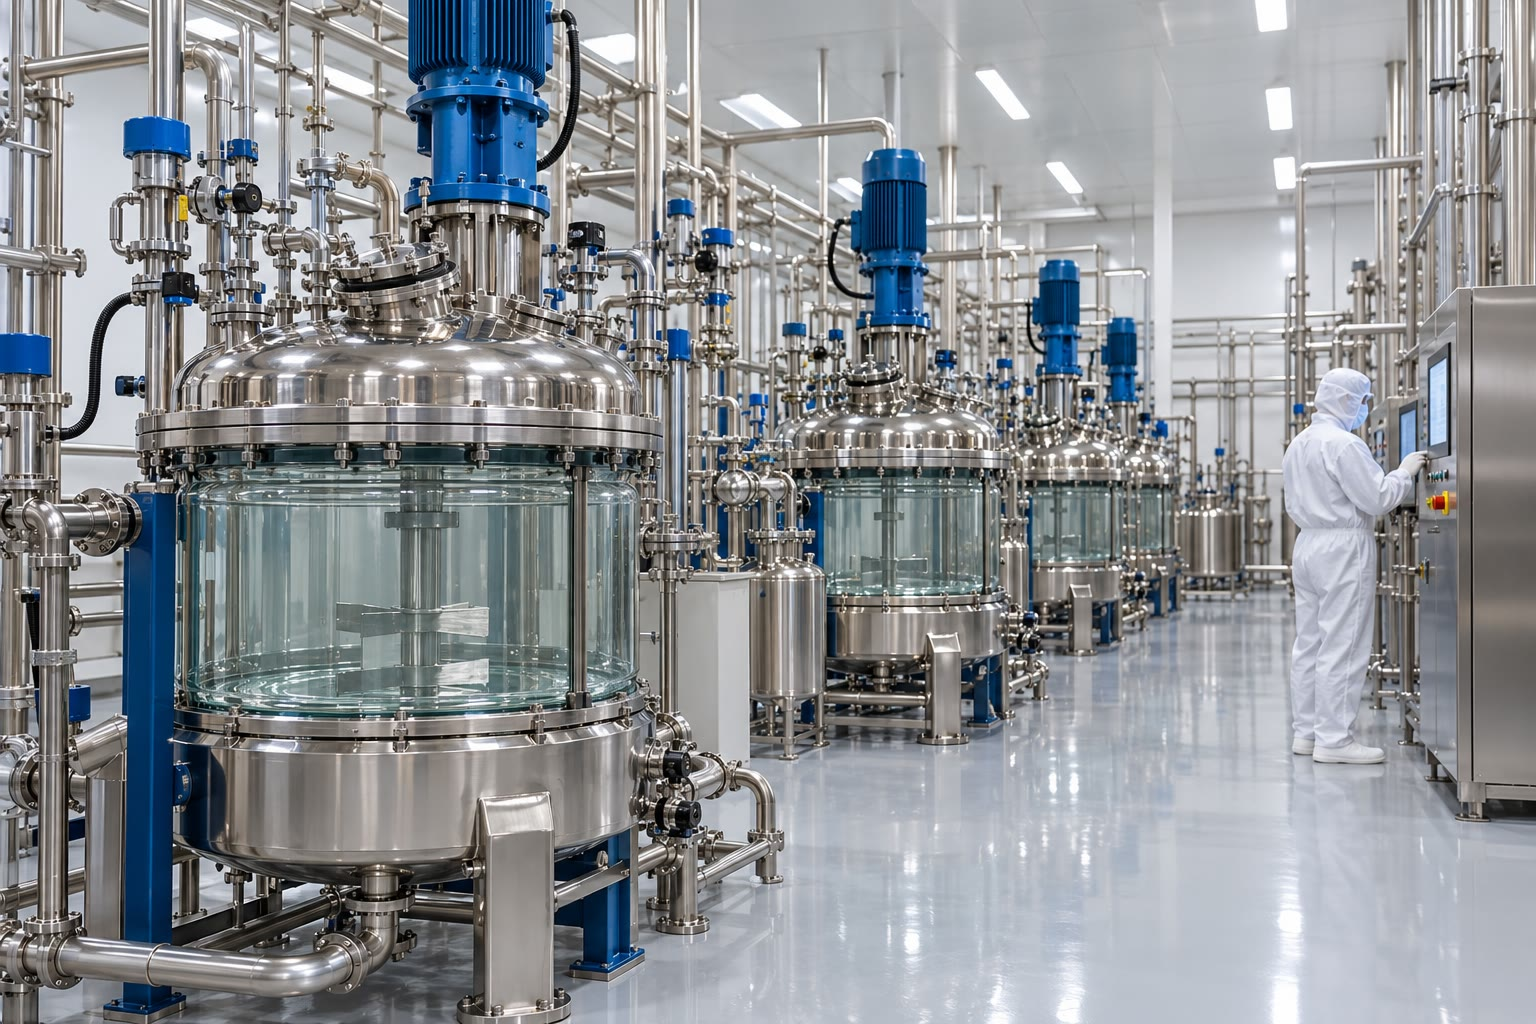
\includegraphics[width=0.58\linewidth]{images/book4/ai/b3-28-api-plant.jpg}

{\small सक्रिय औषधीय अवयव बनाने वाले एक संयंत्र में काँच-अस्तरित रिएक्टरों का एक कक्ष।
इसके अनेक उत्पाद एकल प्रतिबिंबरूपी हैं, जो उत्प्रेरण या विभेदन से बनाए जाते हैं
और किरैल वर्णलेखन से जाँचे जाते हैं।}
\end{omfigure}

\section{प्रतिबिंबरूपी शुद्धता का मापन}

\begin{definition}[प्रतिबिंबरूपी आधिक्य]\label{def:b3:asymmetric-synthesis:ee}
मात्राओं $n_R \ge n_S$ में प्रतिबिंबरूपियों के मिश्रण के लिए \emph{प्रतिबिंबरूपी
आधिक्य}\index{प्रतिबिंबरूपी आधिक्य} $\mathrm{ee} = (n_R - n_S)/(n_R + n_S)$ है और \emph{प्रतिबिंबरूपी अनुपात}
\index{प्रतिबिंबरूपी अनुपात} $\mathrm{er} = n_R/n_S$; अप्रतिबिंबरूपियों के लिए
\emph{अप्रतिबिंबरूपी आधिक्य}\index{अप्रतिबिंबरूपी आधिक्य} de इसी प्रकार
परिभाषित है। \emph{प्रकाशिक शुद्धता}\index{प्रकाशिक शुद्धता} किसी नमूने के विशिष्ट घूर्णन
और शुद्ध प्रतिबिंबरूपी के विशिष्ट घूर्णन का अनुपात है।
\end{definition}

\begin{proposition}[ee और er]\label{prop:b3:asymmetric-synthesis:ee-er}
$\mathrm{ee} = (\mathrm{er} - 1)/(\mathrm{er} + 1)$ और $\mathrm{er} = (1 + \mathrm{ee})/(1 - \mathrm{ee})$।
\end{proposition}

\begin{proof}
$(n_R - n_S)/(n_R + n_S)$ के अंश और हर को $n_S$ से भाग दीजिए; er के लिए हल करने पर
दूसरा रूप मिलता है।
\end{proof}

90\,\% का ee, 95\,:\,5 का er है, 98\,\% का ee, 99\,:\,1 का er। \omterm{def:b3:asymmetric-synthesis:ee}{प्रकाशिक शुद्धता}
ee के बराबर तभी होती है जब घूर्णन संघटन के समानुपाती हो; अशुद्धियाँ,
विलायक, सांद्रता प्रभाव और अनेक यौगिकों के छोटे घूर्णन इसे
अविश्वसनीय बनाते हैं, और ee प्रतिबिंबरूपियों को पृथक करके मापा जाता है।

\begin{method}[किरैल क्रोमैटोग्राम से ee]\label{met:b3:asymmetric-synthesis:ee-chromatogram}
\begin{enumerate}
  \item पहले रेसेमिक मिश्रण अंतःक्षिप्त कीजिए, ताकि दोनों शिखरों की पहचान हो और उनके
        पृथक्करण (आधाररेखा विभेदन) तथा समान क्षेत्रफलों की जाँच हो।
  \item नमूना अंतःक्षिप्त कीजिए और दोनों शिखरों का समाकलन कीजिए।
  \item अकिरैल संसूचक में प्रतिबिंबरूपियों की अनुक्रिया समान होती है, अतः
        $\mathrm{ee} = (A_1 - A_2)/(A_1 + A_2)$; प्रतिबिंबरूपी-शुद्ध मानक से शिखरों का निर्धारण कीजिए।
\end{enumerate}
\end{method}

\begin{omfigure}
\begin{tikzpicture}
\begin{axis}[name=a, width=0.48\linewidth, height=5.4cm, xmin=0, xmax=20, ymin=0, ymax=1.0,
  axis lines=left, xlabel={$\Delta\Delta G^\ddagger$ / \unit{kJ.mol^{-1}}}, ylabel={ee},
  tick label style={font=\scriptsize}, label style={font=\small}]
\addplot[omDef, thick] table[x=ddg, y=eeA] {figdata/out/bachelor-3-er-ddg.dat};
\addplot[omMeth, thick] table[x=ddg, y=eeB] {figdata/out/bachelor-3-er-ddg.dat};
\addplot[omThm, thick] table[x=ddg, y=eeC] {figdata/out/bachelor-3-er-ddg.dat};
\node[font=\scriptsize, omDef, anchor=west] at (axis cs:10,0.55) {\qty{-78}{\celsius}};
\node[font=\scriptsize, omMeth, anchor=west] at (axis cs:10,0.43) {\qty{0}{\celsius}};
\node[font=\scriptsize, omThm, anchor=west] at (axis cs:10,0.31) {\qty{25}{\celsius} (सबसे निचला वक्र)};
\end{axis}
\begin{axis}[at={(a.east)}, anchor=west, xshift=1.4cm, width=0.48\linewidth, height=5.4cm,
  xmin=7.5, xmax=9.5, ymin=0, axis lines=left, ytick=\empty,
  xlabel={प्रतिधारण काल / min}, ylabel={संसूचक संकेत},
  tick label style={font=\scriptsize}, label style={font=\small}]
\addplot[black, thick] table[x=t, y=y] {figdata/out/bachelor-3-er-ddg-b.dat};
\node[font=\scriptsize, anchor=south west] at (axis cs:8.3,250) {(\textit{R}): 97.5};
\node[font=\scriptsize, anchor=south] at (axis cs:9.1,20) {(\textit{S}): 2.5};
\end{axis}
\end{tikzpicture}

{\small बाएँ: \omterm{def:b3:asymmetric-synthesis:ee}{प्रतिबिंबरूपी आधिक्य}, दोनों प्रतिस्पर्धी पथों की \omterm{def:b3:rate-theories:activation}{सक्रियण गिब्स ऊर्जा} के
अंतर के विरुद्ध, तीन तापों पर: वही
$\Delta\Delta G^\ddagger$ निम्न ताप पर अधिक ee देता है। दाएँ: एक किरैल HPLC क्रोमैटोग्राम,
शिखर क्षेत्रफल 97.5 और 2.5 (मॉडल): ee 95\,\%।}
\end{omfigure}

NMR प्रतिबिंबरूपियों में अंतर केवल किरैल परिवेश में करता है: एक किरैल विलायकन
कारक अल्पजीवी अप्रतिबिंबरूपी संकुल बनाता है जिनके संकेत भिन्न होते हैं, और
मॉशर अम्ल के साथ अपने दो अप्रतिबिंबरूपी एस्टरों में बदला गया कोई किरैल ऐल्कोहॉल या ऐमीन
विस्थापन अंतरों के पैटर्न से विन्यास दिखाता है।

\begin{method}[मॉशर एस्टरों से विन्यास, रूपरेखा में]\label{met:b3:asymmetric-synthesis:mosher}
\begin{enumerate}
  \item ऐल्कोहॉल के (\textit{R})- और (\textit{S})-MTPA दोनों एस्टर बनाइए।
  \item उनके प्रोटॉन स्पेक्ट्रम अभिलिखित कीजिए और कार्बिनॉल कार्बन के प्रत्येक ओर के प्रोटॉनों के लिए
        $\Delta\delta = \delta_S - \delta_R$ परिकलित कीजिए।
  \item वरीय संरूपण में अम्ल का फ़ेनिल वलय एक ओर को परिरक्षित करता है:
        $\Delta\delta > 0$ वाले प्रोटॉन एक ओर होते हैं, $\Delta\delta < 0$ वाले दूसरी ओर, जिससे
        दोनों प्रतिस्थापियों का स्थान तय होता है और विन्यास मिलता है।
\end{enumerate}
\end{method}

\section{टॉपिसिटी और त्रिविमवरणात्मक योग}

\begin{definition}[त्रिविमवरणात्मक अभिक्रियाएँ]\label{def:b3:asymmetric-synthesis:selective}
\emph{प्रतिबिंबवरणात्मक अभिक्रिया}\index{प्रतिबिंबवरणात्मक अभिक्रिया} किसी उत्पाद का एक
प्रतिबिंबरूपी दूसरे से अधिक मात्रा में बनाती है; \emph{अप्रतिबिंबवरणात्मक
अभिक्रिया}\index{अप्रतिबिंबवरणात्मक अभिक्रिया} एक अप्रतिबिंबरूपी अधिक मात्रा में बनाती है।
\end{definition}

\begin{definition}[टॉपिसिटी]\label{def:b3:asymmetric-synthesis:topicity}
किसी अणु के दो समूह \emph{समरूपस्थ}\index{समरूपस्थ} होते हैं जब
अणु के घूर्णन द्वारा परस्पर बदले जाते हैं (किसी को भी प्रतिस्थापित करने से वही यौगिक मिलता है),
\emph{प्रतिबिंबस्थ}\index{प्रतिबिंबस्थ} जब केवल परावर्तन द्वारा परस्पर बदले जाते हैं
(एक या दूसरे को प्रतिस्थापित करने से प्रतिबिंबरूपी मिलते हैं), और
\emph{अप्रतिबिंबस्थ}\index{अप्रतिबिंबस्थ} जब कोई \omterm{def:b3:point-groups:operation}{सममिति संक्रिया} उन्हें परस्पर
नहीं बदलती (एक या दूसरे को प्रतिस्थापित करने से अप्रतिबिंबरूपी मिलते हैं)।
\end{definition}

त्रिविमजनक केंद्र के बगल वाले $\ce{CH2}$ समूह के दोनों हाइड्रोजन \omterm{def:b3:asymmetric-synthesis:topicity}{अप्रतिबिंबस्थ} होते हैं: उनके
रासायनिक विस्थापन भिन्न होते हैं और वे एक-दूसरे से युग्मित होते हैं, इसीलिए ऐसा
समूह NMR में प्रायः दो संकेतों के रूप में दिखता है।

\begin{definition}[पूर्वकिरैल फलक]\label{def:b3:asymmetric-synthesis:faces}
तीन भिन्न प्रतिस्थापियों वाला त्रिकोणीय कार्बन \emph{पूर्वकिरैल}\index{पूर्वकिरैल} होता है:
किसी चौथे, भिन्न समूह का योग एक त्रिविमजनक केंद्र बनाता है। घटती CIP प्राथमिकता में
तीनों प्रतिस्थापियों को दक्षिणावर्त चलता हुआ दिखाने वाला उसका फलक
\emph{Re फलक}\index{Re फलक} है; वामावर्त, \emph{Si फलक}\index{Si फलक}।
\end{definition}

\begin{omfigure}
\begin{tikzpicture}[font=\small, >=Stealth]
  \coordinate (c) at (0,0);
  \draw[thick, double, double distance=1.6pt] (c) -- (90:1.1) node[above] {O (1)};
  \draw[thick] (c) -- (210:1.1) node[below left] {$\ce{C6H5}$ (2)};
  \draw[thick] (c) -- (330:1.1) node[below right] {$\ce{CH3}$ (3)};
  \fill (c) circle (1.6pt);
  \draw[->, thick, omThm] (70:0.6) arc[start angle=70, end angle=200, radius=0.6];
  \node[font=\scriptsize, omThm, align=center] at (-1.9,0.75) {1 $\to$ 2 $\to$ 3\\ वामावर्त:\\ \textit{Si} फलक};
  \node[font=\scriptsize, align=left, anchor=west] at (2.6,0.4) {पाठक की ओर का फलक: \textit{Si}\\ पृष्ठ के पीछे का फलक: \textit{Re}};
  \node[font=\scriptsize, align=left, anchor=west] at (2.6,-0.5) {\textit{Re} फलक से जुड़ा हाइड्राइड\\ (\textit{S})-1-फ़ेनिलएथेनॉल देता है};
\end{tikzpicture}

{\small ऐसीटोफ़ीनोन के फलक। सामने से देखने पर, कार्बोनिल कार्बन के प्रतिस्थापी
CIP क्रम में (O, फ़ेनिल, मेथिल) वामावर्त चलते हैं: सामने का
फलक \textit{Si} है, पीछे का फलक \textit{Re}।}
\end{omfigure}

\begin{method}[Re और Si फलकों का निर्धारण]\label{met:b3:asymmetric-synthesis:re-si}
\begin{enumerate}
  \item त्रिकोणीय परमाणु के तीनों प्रतिस्थापियों को CIP नियमों से क्रम दीजिए (एक
        द्विबंध अपने साथी को दो बार गिनता है)।
  \item रुचि के फलक को देखिए, त्रिकोणीय तल पृष्ठ के तल में रखकर।
  \item दक्षिणावर्त 1 $\to$ 2 $\to$ 3: \textit{Re}; वामावर्त: \textit{Si}।
  \item उत्पाद का नाम देने के लिए नया समूह दर्शक की ओर जोड़िए और
        नए त्रिविमजनक केंद्र पर CIP नियम लागू कीजिए; Re आक्रमण सदैव \textit{R} नहीं देता।
\end{enumerate}
\end{method}

\begin{definition}[फ़ेल्किन--आन मॉडल और कीलेटन नियंत्रण]\label{def:b3:asymmetric-synthesis:felkin}
\emph{फ़ेल्किन--आन मॉडल}\index{फ़ेल्किन--आन मॉडल} त्रिविमजनक केंद्र के बगल वाले
कार्बोनिल समूह पर नाभिकरागी योग के मुख्य
अप्रतिबिंबरूपी का पूर्वानुमान करता है: उस केंद्र पर सबसे बड़ा समूह
कार्बोनिल तल के लंबवत होता है, और नाभिकरागी उसके anti, सबसे छोटे
समूह के पास से, बुर्गी--डुनिट्ज़ प्रक्षेप-पथ के अनुदिश, पहुँचता है। \emph{कीलेटन
नियंत्रण}\index{कीलेटन नियंत्रण} में कार्बोनिल ऑक्सीजन और त्रिविमजनक केंद्र पर स्थित
एक दाता समूह, दोनों से बँधा एक धातु आयन संरूपण को स्थिर कर देता है, और
नाभिकरागी कीलेट वलय के कम बाधित फलक पर जुड़ता है।
\end{definition}

\begin{proposition}[फ़ेल्किन--आन वरणात्मकता]\label{prop:b3:asymmetric-synthesis:felkin}
कीलेटकारी समूह-रहित किसी $\alpha$-किरैल ऐल्डिहाइड या कीटोन के लिए मुख्य
उत्पाद वही होता है जिसका पूर्वानुमान \omterm{def:b3:asymmetric-synthesis:felkin}{फ़ेल्किन--आन मॉडल} करता है (एक आनुभविक मॉडल,
परिकलन द्वारा समर्थित)। \admitted
\end{proposition}

\begin{omfigure}
\begin{tikzpicture}[font=\small, >=Stealth]
  \foreach \a/\lab in {90/L, 330/M, 210/S} {
    \draw[line width=0.8pt] (\a:0.55) -- (\a:1.1) node[pos=1.3] {\lab};
  }
  \fill[white] (0,0) circle (0.55);
  \draw[line width=0.8pt] (0,0) circle (0.55);
  \draw[line width=0.8pt, double, double distance=1.4pt] (0,0) -- (0:1.1) node[right] {O};
  \draw[line width=0.8pt] (0,0) -- (180:1.1) node[left] {R};
  \draw[->, very thick, omThm] (250:2.2) -- (250:0.25);
  \node[omThm, anchor=north] at (250:2.25) {Nu$^-$};
  \node[font=\scriptsize, align=left, anchor=west] at (1.7,-1.0) {Nu$^-$ L के anti प्रवेश करता है,\\ S के पास से, C=O आबंध से\\ लगभग 107° पर};
\end{tikzpicture}

{\small \omterm{def:b3:asymmetric-synthesis:felkin}{फ़ेल्किन--आन मॉडल}, कार्बोनिल कार्बन (सामने, O और R से
आबंध) से त्रिविमजनक केंद्र (पीछे का वृत्त, समूह L, M और S) तक के आबंध के अनुदिश देखा गया।
बड़ा समूह कार्बोनिल तल के लंबवत है; नाभिकरागी
विपरीत ओर से, छोटे समूह के निकट और ऑक्सीजन से दूर, आता है।}
\end{omfigure}

\section{रणनीतियाँ}

\begin{definition}[किरैल कुंड]\label{def:b3:asymmetric-synthesis:chiral-pool}
\emph{किरैल कुंड}\index{किरैल कुंड} सस्ते, प्रतिबिंबरूपी-शुद्ध
प्राकृतिक यौगिकों (ऐमीनो अम्ल, शर्कराएँ, टर्पीन, हाइड्रॉक्सी अम्ल) का वह समुच्चय है जिसका उपयोग
प्रारंभिक पदार्थों के रूप में होता है, उनके त्रिविमजनक केंद्र लक्ष्य में ले जाए जाते हैं।
\end{definition}

\begin{definition}[किरैल सहायक]\label{def:b3:asymmetric-synthesis:auxiliary}
\emph{किरैल सहायक}\index{किरैल सहायक} एक प्रतिबिंबरूपी-शुद्ध समूह है जिसे
किसी अभिक्रिया के त्रिविम रसायन के नियंत्रण के लिए किसी क्रियाधार से अस्थायी रूप से जोड़ा जाता है,
फिर हटाकर पुनः प्राप्त किया जाता है।
\end{definition}

इवान्स ऐल्किलनों में ऐमीनो अम्ल से बने एक ऑक्साज़ोलिडिनोन का ऐसिलन किया जाता है;
लिथियम या सोडियम ईनोलेट, सहायक के कार्बोनिल समूह से कीलेटित, पर
किसी ऐल्किल हैलाइड द्वारा सहायक के प्रतिस्थापी से दूर वाले फलक पर आक्रमण होता है,
जिससे एक अप्रतिबिंबरूपी मिलता है, प्रायः 95\,\% से ऊपर de के साथ; फिर जल-अपघटन
किरैल अम्ल और सहायक को मुक्त करता है।

\begin{definition}[विभेदन]\label{def:b3:asymmetric-synthesis:resolution}
\emph{रेसेमिक विभेदन}\index{रेसेमिक विभेदन} किसी रेसेमिक मिश्रण का
प्रतिबिंबरूपियों में पृथक्करण है, पारंपरिक रूप से किसी प्रतिबिंबरूपी-शुद्ध अम्ल या क्षारक के साथ
अप्रतिबिंबरूपी लवणों के क्रिस्टलन द्वारा। \emph{बलगतिक विभेदन}\index{बलगतिक विभेदन}
में दोनों प्रतिबिंबरूपी किसी किरैल अभिकर्मक या
उत्प्रेरक के साथ भिन्न दरों से अभिक्रिया करते हैं, वरणात्मकता $s = k_{\mathrm{fast}}/k_{\mathrm{slow}}$ के साथ। \emph{गतिशील बलगतिक
विभेदन}\index{गतिशील बलगतिक विभेदन} में क्रियाधार के प्रतिबिंबरूपी
तेज़ी से परस्पर रूपांतरित होते रहते हैं जबकि उनमें से एक अभिक्रिया करता है।
\end{definition}

\begin{theorem}[कागान समीकरण]\label{thm:b3:asymmetric-synthesis:kagan}
वरणात्मकता $s$ वाली प्रथम-कोटि अभिक्रियाओं द्वारा किसी रेसेमिक मिश्रण के \omterm{def:b3:asymmetric-synthesis:resolution}{बलगतिक विभेदन} में
रूपांतरण $c$ और शेष क्रियाधार का ee इस प्रकार संबंधित हैं
\[
  s = \frac{\ln[(1 - c)(1 - \mathrm{ee})]}{\ln[(1 - c)(1 + \mathrm{ee})]}.
\]
\end{theorem}

\begin{proof}
प्रत्येक प्रतिबिंबरूपी चरघातांकी रूप से क्षयित होता है: शेष अंश $f_1 = \eu^{-k_{\mathrm{fast}}t}$ और
$f_2 = \eu^{-k_{\mathrm{slow}}t}$ हैं, अतः $\ln f_1 = s\ln f_2$। समान मात्राओं से आरंभ करने पर $1 - c = (f_1 + f_2)/2$ और
$\mathrm{ee} = (f_2 - f_1)/(f_1 + f_2)$। तब $(1 - c)(1 - \mathrm{ee}) = \tfrac12(f_1 + f_2)\cdot 2f_1/(f_1 + f_2) = f_1$ और इसी प्रकार
$(1 - c)(1 + \mathrm{ee}) = f_2$। अतः $s = \ln f_1/\ln f_2$ बताया गया अनुपात है।
\end{proof}

\begin{omfigure}
\begin{tikzpicture}
\begin{axis}[width=0.62\linewidth, height=5.6cm, xmin=0, xmax=1, ymin=0, ymax=1.02,
  axis lines=left, xlabel={रूपांतरण $c$}, ylabel={ee},
  tick label style={font=\scriptsize}, label style={font=\small},
  legend style={font=\scriptsize, draw=none, at={(1.04,0.5)}, anchor=west}, legend cell align=left]
\addplot[color=omThm, thick] table[x=c, y=eesm] {figdata/out/bachelor-3-kinetic-resolution-s2.dat};
\addlegendentry{$s = 2$}
\addplot[color=omMeth, thick] table[x=c, y=eesm] {figdata/out/bachelor-3-kinetic-resolution-s10.dat};
\addlegendentry{$s = 10$}
\addplot[color=omDef, thick] table[x=c, y=eesm] {figdata/out/bachelor-3-kinetic-resolution-s50.dat};
\addlegendentry{$s = 50$}
\addplot[color=omThm, thick, dashed] table[x=c, y=eep] {figdata/out/bachelor-3-kinetic-resolution-s2.dat};
\addplot[color=omMeth, thick, dashed] table[x=c, y=eep] {figdata/out/bachelor-3-kinetic-resolution-s10.dat};
\addplot[color=omDef, thick, dashed] table[x=c, y=eep] {figdata/out/bachelor-3-kinetic-resolution-s50.dat};
\end{axis}
\end{tikzpicture}

{\small \omterm{def:b3:asymmetric-synthesis:resolution}{बलगतिक विभेदन}: शेष क्रियाधार (ठोस) और
उत्पाद (धराशायी) का ee, रूपांतरण के विरुद्ध, तीन वरणात्मकताओं के लिए। क्रियाधार को
पर्याप्त आगे जाकर, लब्धि की कीमत पर, सदैव प्रतिबिंबरूपी-शुद्ध बनाया जा सकता है;
उत्पाद निम्न रूपांतरण पर सबसे शुद्ध होता है।}
\end{omfigure}

\begin{proposition}[गतिशील बलगतिक विभेदन]\label{prop:b3:asymmetric-synthesis:dkr}
यदि क्रियाधार के प्रतिबिंबरूपी किसी के भी अभिक्रिया करने से कहीं तेज़ी से परस्पर रूपांतरित हों, तो
पूरा रेसेमिक मिश्रण एक उत्पाद प्रतिबिंबरूपी में बदला जा सकता है, $s$ द्वारा तय ee के साथ:
$\mathrm{er} = s$।
\end{proposition}

\begin{proof}
तीव्र रेसेमीकरण क्रियाधार के दोनों प्रतिबिंबरूपियों को हर समय समान मात्राओं में
रखता है। तब उत्पाद $k_{\mathrm{fast}}[\mathrm A] : k_{\mathrm{slow}}[\mathrm A] = s$ अनुपात वाली दरों पर बनते हैं, और
सारे क्रियाधार के, मुख्यतः तीव्र प्रतिबिंबरूपी के माध्यम से, उपभुक्त होने से पहले अभिक्रिया को कुछ नहीं
रोकता: लब्धि 100\,\% तक पहुँच सकती है, $\mathrm{er} = s$ के साथ।
\end{proof}

\begin{method}[रणनीति का चयन]\label{met:b3:asymmetric-synthesis:strategy}
\begin{enumerate}
  \item यदि लक्ष्य के त्रिविमजनक केंद्र किसी सस्ते प्राकृतिक यौगिक में विद्यमान हों, तो
        \omterm{def:b3:asymmetric-synthesis:chiral-pool}{किरैल कुंड} से आरंभ कीजिए।
  \item एक बार के संश्लेषण के लिए, या किसी कार्बोनिल समूह के बगल में केंद्र को विश्वसनीय रूप से स्थापित करने के लिए,
        दो अतिरिक्त चरणों की कीमत पर, सहायक का उपयोग कीजिए।
  \item यदि रेसेमिक मिश्रण सस्ता हो और अवांछित प्रतिबिंबरूपी का पुनर्चक्रण या
        रेसेमीकरण हो सके, तो उसका विभेदन कीजिए (पारंपरिक, बलगतिक या गतिशील)।
  \item बड़े पैमाने के लिए असममित उत्प्रेरक खोजिए: प्रति उत्प्रेरकी आवर्त एक त्रिविमजनक केंद्र,
        कोई रससमीकरणमितीय किरैल अपशिष्ट नहीं।
\end{enumerate}
\end{method}

\section{धातुओं के साथ असममित उत्प्रेरण}

\begin{definition}[असममित उत्प्रेरण]\label{def:b3:asymmetric-synthesis:asymmetric-catalysis}
\emph{असममित उत्प्रेरण}\index{असममित उत्प्रेरण} कम मात्रा में प्रयुक्त किरैल उत्प्रेरक के साथ
प्रतिबिंबवरणात्मक संश्लेषण है; धातु उत्प्रेरकों में
किरैलता प्रायः किसी \emph{किरैल लिगैंड}\index{किरैल लिगैंड} से आती है।
\end{definition}

\begin{theorem}[ऊर्जा से वरणात्मकता]\label{thm:b3:asymmetric-synthesis:er-ddg}
यदि दो प्रतिबिंबरूपी उत्पाद अप्रतिबिंबरूपी संक्रमण अवस्थाओं से होकर,
समान पूर्व-घातांकी गुणकों के साथ, अनुत्क्रमणीय रूप से, बलगतिक नियंत्रण में बनें, तो
$\mathrm{er} = \exp(\Delta\Delta G^\ddagger/RT)$, जहाँ $\Delta\Delta G^\ddagger$ उनकी सक्रियण गिब्स ऊर्जाओं का
अंतर है।
\end{theorem}

\begin{proof}
\omterm{thm:b3:rate-theories:eyring}{आयरिंग समीकरण} (\cref{ch:b3:rate-theories}) से
$k_i = (k_BT/h)\eu^{-\Delta G_i^\ddagger/RT}$; दोनों उत्पाद उन्हीं अभिकारकों से बनते हैं, अतः हर क्षण
उनकी दरें $k_1/k_2 = \eu^{(\Delta G_2^\ddagger - \Delta G_1^\ddagger)/RT}$ अनुपात में होती हैं, और बनी मात्राएँ भी।
\end{proof}

\qty{25}{\celsius} पर 99\,\% ee (er 199) के लिए $\Delta\Delta G^\ddagger = RT\ln 199 = \qty{13.1}{kJ/mol}$ चाहिए, लगभग एक
हाइड्रोजन आबंध की ऊर्जा; \qty{-78}{\celsius} पर \qty{8.6}{kJ/mol} पर्याप्त है।

\begin{proposition}[$C_2$-सममित लिगैंड]\label{prop:b3:asymmetric-synthesis:c2}
$C_2$-सममित \omterm{def:b3:asymmetric-synthesis:asymmetric-catalysis}{किरैल लिगैंड} तुलना की जाने वाली अप्रतिबिंबरूपी संक्रमण
अवस्थाओं की संख्या आधी कर देता है, क्योंकि उसके द्वारा छोड़े गए दोनों उपसहसंयोजन स्थल
तुल्य होते हैं।
\end{proposition}

\begin{proof}
उत्प्रेरक का $C_2$ घूर्णन एक मुक्त स्थल को दूसरे पर प्रतिचित्रित करता है और
उत्प्रेरक को अपरिवर्तित छोड़ता है; अतः एक स्थल पर कोई भी संक्रमण अवस्था दूसरे स्थल पर
घूर्णित अवस्था के सर्वसम है। केवल एक स्थल पर बंधन विधाओं (क्रियाधार फलक,
अभिविन्यास) की तुलना आवश्यक है।
\end{proof}

नोल्स ने रोडियम के साथ किरैल मोनोफ़ॉस्फ़ीनों, फिर $C_2$-सममित डाइफ़ॉस्फ़ीन DIPAMP, का उपयोग करके
एक इनैमाइड का L-डोपा के संरक्षित ऐमीनो अम्ल में हाइड्रोजनन किया; नोयोरी का BINAP,
रूथेनियम के साथ, कीटोनों और क्रियात्मकीकृत ऐल्कीनों का हाइड्रोजनन करता है, और,
किसी किरैल डाइऐमीन के साथ मिलकर, सरल कीटोनों का अत्यंत ऊँचे ee के साथ। रोडियम इनैमाइड
हाइड्रोजनन में मुख्य उत्पाद कम स्थायी, गौण
उत्प्रेरक--क्रियाधार संकुल से आता है, जो हाइड्रोजन से कहीं तेज़ी से अभिक्रिया करता है:
वरणात्मकता संक्रमण अवस्थाओं पर तय होती है, मध्यवर्तियों की \omterm{def:b3:partition-functions:boltzmann}{समष्टियों} से नहीं
(कर्टिन--हैमेट सिद्धांत)।

\begin{definition}[शार्पलेस एपॉक्सीकरण]\label{def:b3:asymmetric-synthesis:sharpless}
\emph{शार्पलेस एपॉक्सीकरण}\index{शार्पलेस एपॉक्सीकरण} \textit{tert}-ब्यूटिल हाइड्रोपेरॉक्साइड द्वारा
ऐलिलिक ऐल्कोहॉलों का प्रतिबिंबवरणात्मक एपॉक्सीकरण है,
जो प्रतिबिंबरूपी-शुद्ध डाइएथिल टार्ट्रेट के साथ टाइटेनियम(IV) आइसोप्रोपॉक्साइड द्वारा उत्प्रेरित होता है;
ऐल्कोहॉल टाइटेनियम से बँधता है, जो ऑक्सीजन को ऐल्कीन के एक फलक पर पहुँचाता है,
जिसे टार्ट्रेट चुनता है।
\end{definition}

\begin{omfigure}
\begin{tikzpicture}[font=\small, >=Stealth]
  \draw[black!50] (-2.3,-1.55) rectangle (2.5,1.55);
  % C3 (top) = C2 (bottom); C2 carries R1 (left) and CH2OH (lower right),
  % C3 carries R2 (left) and R3 (right)
  \coordinate (c3) at (0,0.45); \coordinate (c2) at (0,-0.45);
  \draw[thick, double, double distance=1.6pt] (c3) -- (c2);
  \draw[thick] (c3) -- (-0.9,0.95) node[above left, inner sep=1pt] {R$^2$};
  \draw[thick] (c3) -- (0.9,0.95) node[above right, inner sep=1pt] {R$^3$};
  \draw[thick] (c2) -- (-0.9,-0.95) node[below left, inner sep=1pt] {R$^1$};
  \draw[thick] (c2) -- (0.9,-0.95) node[below right, inner sep=1pt] {$\ce{CH2OH}$};
  \draw[->, very thick, omDef] (0.35,2.5) -- (0.2,0.1) node[pos=0, above, align=center, font=\scriptsize] {D-($-$)-डाइएथिल टार्ट्रेट:\\ ऊपरी फलक से O};
  \draw[->, very thick, omThm] (0.35,-2.6) -- (0.2,-0.1) node[pos=0, below, align=center, font=\scriptsize] {L-($+$)-डाइएथिल टार्ट्रेट:\\ निचले फलक से O};
\end{tikzpicture}

{\small शार्पलेस का स्मृति-सूत्र। ऐलिलिक ऐल्कोहॉल को तल में बनाने पर, जिसमें
$\ce{CH2OH}$ समूह नीचे दाईं ओर हो, L-($+$)-डाइएथिल टार्ट्रेट ऑक्सीजन को
तल के नीचे से और D-($-$)-डाइएथिल टार्ट्रेट ऊपर से पहुँचाता है,
प्रतिस्थापी $\mathrm R^1$ से $\mathrm R^3$ चाहे जो हों।}
\end{omfigure}

यही विचार, एक सस्ते प्राकृतिक लिगैंड द्वारा किरैल जेब में थामी गई धातु, ऑस्मियम और सिनकोना
ऐल्कलॉइड लिगैंडों के साथ ऐल्कीनों का शार्पलेस असममित डाइहाइड्रॉक्सिलन देता है।
जब लिगैंड प्रतिबिंबरूपी-शुद्ध न हो, तो उत्पाद के ee का लिगैंड के ee के
समानुपाती होना आवश्यक नहीं: दो लिगैंडों के समुच्चय, जिनकी
समकिरैल और विषमकिरैल युग्मों के लिए सक्रियताएँ भिन्न होती हैं, अरैखिक
प्रभाव देते हैं, जो कभी-कभी उपयोगी प्रवर्धन होते हैं।

\section{कार्बनिक उत्प्रेरण}

\begin{definition}[कार्बनिक उत्प्रेरण]\label{def:b3:asymmetric-synthesis:organocatalysis}
\emph{कार्बनिक उत्प्रेरण}\index{कार्बनिक उत्प्रेरण} धातुओं के बिना छोटे कार्बनिक
अणुओं द्वारा उत्प्रेरण है। \emph{एनामीन उत्प्रेरण}\index{एनामीन उत्प्रेरण} में
एक द्वितीयक ऐमीन किसी कीटोन या ऐल्डिहाइड को एक नाभिकरागी एनामीन में बदल देती है;
\emph{इमीनियम उत्प्रेरण}\index{इमीनियम उत्प्रेरण} में वह किसी $\alpha,\beta$-असंतृप्त
ऐल्डिहाइड को घटे हुए LUMO वाले एक इलेक्ट्रॉनरागी इमीनियम आयन में बदल देती है।
\end{definition}

\begin{omfigure}
\begin{tikzpicture}[font=\small]
  % proline-derived enamine and the aldehyde held by the carboxylic acid
  \coordinate (n) at (0,0.7); \coordinate (r2) at (0.67,0.22); \coordinate (r3) at (0.41,-0.57);
  \coordinate (r4) at (-0.41,-0.57); \coordinate (r5) at (-0.67,0.22);
  \draw[thick] (n) -- (r2) -- (r3) -- (r4) -- (r5) -- (n);
  \node[fill=white, inner sep=0.6pt] at (n) {N};
  \coordinate (ca) at (0,1.45); \coordinate (cb) at (0.72,1.85);
  \draw[thick] (0,0.88) -- (ca);
  \draw[thick] (ca) -- (-0.62,1.85) node[left, inner sep=1pt] {$\ce{CH3}$};
  \draw[thick, double, double distance=1.5pt] (ca) -- (cb);
  \coordinate (cacid) at (1.45,0.45);
  \draw[thick] (r2) -- (cacid);
  \draw[thick, double, double distance=1.5pt] (cacid) -- (1.75,-0.15) node[below, inner sep=1pt] {O};
  \draw[thick] (cacid) -- (2.05,0.9) node[right, inner sep=1pt] (oh) {O--H};
  \node (cald) at (1.55,2.55) {C};
  \draw[thick, double, double distance=1.5pt] (cald) -- (2.35,2.15) node[right, inner sep=1pt] (oald) {O};
  \draw[thick] (cald) -- (1.3,3.15) node[above, inner sep=1pt] {R};
  \draw[omThm, thick, densely dashed] (cb) -- (cald);
  \draw[omMeth, thick, dotted] (2.45,1.05) -- (2.5,2.0);
  \node[font=\scriptsize, omThm, anchor=east] at (1.05,2.35) {C--C बनता है};
  \node[font=\scriptsize, omMeth, anchor=west] at (2.6,1.55) {H आबंध};
\end{tikzpicture}

{\small प्रोलीन-उत्प्रेरित ऐल्डोल अभिक्रिया, व्यवस्थात्मक संक्रमण अवस्था:
ऐसीटोन और पिरोलिडीन नाइट्रोजन से बना एनामीन ऐल्डिहाइड पर आक्रमण करता है,
जिसका ऑक्सीजन उत्प्रेरक के कार्बोक्सिलिक अम्ल से एक हाइड्रोजन आबंध द्वारा थामा जाता है;
वह आबंध तय करता है कि ऐल्डिहाइड के किस फलक पर आक्रमण होता है।}
\end{omfigure}

प्रोलीन, एक सस्ता ऐमीनो अम्ल, ऊँचे ee के साथ ट्राइकीटोनों की अंतःआण्विक ऐल्डोल अभिक्रियाओं को
उत्प्रेरित करता है (हायोश--पैरिश और वीलैंड--मीशर कीटोन, जो
1970 के दशक से स्टेरॉयड संश्लेषणों में प्रयुक्त होते हैं) और, जैसा 2000 में दिखाया गया, ऐल्डिहाइडों के साथ
ऐसीटोन की अंतराआण्विक ऐल्डोल अभिक्रियाओं को भी। किरैल इमिडैज़ोलिडिनोन
डील्स--ऐल्डर अभिक्रियाओं और संयुग्मी योगों में इमीनियम आयनों के माध्यम से कार्य करते हैं; किरैल
फ़ॉस्फ़ोरिक अम्ल, किरैल जेब वाले प्रबल ब्रॉन्स्टेड अम्ल, इमीनों को
प्रोटॉनन द्वारा सक्रियित करते हैं। कार्बनिक उत्प्रेरक वायु और जल में स्थायी हैं और उत्पाद में कोई धातु
नहीं छोड़ते।

\begin{inthelab}[एक किरैल HPLC विश्लेषण]
एक किरैल स्तंभ, सेलुलोस या ऐमाइलोस व्युत्पन्न से लेपित सिलिका, को
हेक्सेन--आइसोप्रोपेनॉल मिश्रण से साम्यित किया जाता है। पहले रेसेमिक मिश्रण अंतःक्षिप्त किया जाता है
और विलायक अनुपात तब तक समायोजित किया जाता है जब तक दोनों शिखर आधाररेखा तक पृथक न हो जाएँ; फिर
उत्क्षालक में लगभग एक मिलीग्राम प्रति मिलीलीटर पर घुला नमूना
अंतःक्षिप्त किया जाता है, और उस तरंगदैर्ध्य पर जहाँ दोनों अवशोषित करते हैं, शिखरों का समाकलन किया जाता है।
\end{inthelab}

\begin{safety}{\ghs[0.6cm]{GHS02}\ghs[0.6cm]{GHS05}\ghs[0.6cm]{GHS06}\ghs[0.6cm]{GHS08}\ghs[0.6cm]{GHS09}}
% ledger: ghs4:TBHP, ghs4:TiOiPr4
\textit{tert}-ब्यूटिल हाइड्रोपेरॉक्साइड: ज्वलनशील, गर्म करने पर स्वतःक्रियाशील, त्वचा के संपर्क में
विषैला, संक्षारक, सुग्राहीकारी, आनुवंशिक दोष उत्पन्न करने का संदेह; इसे
विलयन के रूप में प्रयुक्त किया जाता है, ठंडा रखा जाता है, कभी सांद्रित नहीं किया जाता, और कार्य-समापन से पहले
अतिरिक्त पेरॉक्साइड नष्ट कर दिया जाता है। टाइटेनियम(IV) आइसोप्रोपॉक्साइड: ज्वलनशील, उत्तेजक,
नमी से विघटित।
\end{safety}

\begin{history}[असममित उत्प्रेरण के लिए दो पुरस्कार]
विलियम नोल्स, र्योजी नोयोरी और बैरी शार्पलेस ने किरैलतः उत्प्रेरित हाइड्रोजननों और ऑक्सीकरणों के लिए
रसायन का 2001 का नोबेल पुरस्कार साझा किया। बेंजामिन लिस्ट
और डेविड मैकमिलन, जिन्होंने 2000 में दिखाया था कि छोटे कार्बनिक अणु
धातु संकुलों जितनी व्यापकता से \omterm{def:b3:asymmetric-synthesis:selective}{प्रतिबिंबवरणात्मक अभिक्रियाओं} को उत्प्रेरित कर सकते हैं, को
2021 का पुरस्कार मिला।
\end{history}

\section{अभ्यास}

\begin{exercise}[$\star$]\label{exo:b3:asymmetric-synthesis:1}
बदलिए: ee 80\,\% को er में; er 99\,:\,1 को ee में; ee 50\,\% को प्रत्येक
प्रतिबिंबरूपी के प्रतिशत में।
\end{exercise}

\begin{exercise}[$\star$]\label{exo:b3:asymmetric-synthesis:2}
एक किरैल HPLC अनुरेख दोनों प्रतिबिंबरूपियों के लिए 1840 और 60 क्षेत्रफल के शिखर दिखाता है।
ee परिकलित कीजिए।
\end{exercise}

\begin{exercise}[$\star$]\label{exo:b3:asymmetric-synthesis:3}
प्रोपेनैल के कार्बोनिल कार्बन के Re और \omterm{def:b3:asymmetric-synthesis:faces}{Si फलकों} का निर्धारण कीजिए, और \omterm{def:b3:asymmetric-synthesis:faces}{Re फलक} पर मेथिल नाभिकरागी के
योग से बने ऐल्कोहॉल का नाम बताइए।
\end{exercise}

\begin{exercise}[$\star$]\label{exo:b3:asymmetric-synthesis:4}
एथेनॉल के दोनों मेथिलीन प्रोटॉन \omterm{def:b3:asymmetric-synthesis:topicity}{समरूपस्थ}, \omterm{def:b3:asymmetric-synthesis:topicity}{प्रतिबिंबस्थ} या \omterm{def:b3:asymmetric-synthesis:topicity}{अप्रतिबिंबस्थ} हैं?
और 2-ब्यूटेनॉल के $\ce{CH2}$ समूह के प्रोटॉन?
\end{exercise}

\begin{exercise}[$\star\star$]\label{exo:b3:asymmetric-synthesis:5}
\qty{25}{\celsius} और \qty{-78}{\celsius} पर 99\,\% ee के लिए आवश्यक $\Delta\Delta G^\ddagger$ परिकलित कीजिए, और \qty{-78}{\celsius} पर
उस उत्प्रेरक द्वारा दिया गया ee जो \qty{25}{\celsius} पर 80\,\% ee देता है (वही $\Delta\Delta G^\ddagger$)।
\end{exercise}

\begin{exercise}[$\star\star$]\label{exo:b3:asymmetric-synthesis:6}
किसी ऐमीन के एक नमूने के लिए $[\alpha]_D = -12.0$ है, उन परिस्थितियों में जहाँ शुद्ध (\textit{S})
प्रतिबिंबरूपी का $-15.0$ है (अभ्यास के आँकड़े)। इसकी \omterm{def:b3:asymmetric-synthesis:ee}{प्रकाशिक शुद्धता} और
प्रतिबिंबरूपियों के प्रतिशत बताइए, घूर्णन को संघटन के समानुपाती मानकर।
यह मापन वर्णलेखन से कम विश्वसनीय क्यों है?
\end{exercise}

\begin{exercise}[$\star\star$]\label{exo:b3:asymmetric-synthesis:7}
किसी रेसेमिक ऐल्कोहॉल के लाइपेज़-उत्प्रेरित ऐसीटिलन में शेष ऐल्कोहॉल
का ee 60\,\% रूपांतरण पर 90\,\% है। $s$ परिकलित कीजिए।
\end{exercise}

\begin{exercise}[$\star\star$]\label{exo:b3:asymmetric-synthesis:8}
(\textit{E})-हेक्स-2-ईन-1-ऑल से L-($+$)-डाइएथिल टार्ट्रेट के साथ, और
D-($-$)-डाइएथिल टार्ट्रेट के साथ, बनने वाले एपॉक्साइड का पूर्वानुमान कीजिए।
\end{exercise}

\begin{exercise}[$\star\star$]\label{exo:b3:asymmetric-synthesis:9}
(\textit{S})-2-फ़ेनिलप्रोपेनैल को मेथिलमैग्नीशियम ब्रोमाइड से उपचारित किया जाता है। \omterm{def:b3:asymmetric-synthesis:felkin}{फ़ेल्किन--आन
मॉडल} से मुख्य अप्रतिबिंबरूपी का पूर्वानुमान कीजिए।
\end{exercise}

\begin{exercise}[$\star\star\star$]\label{exo:b3:asymmetric-synthesis:10}
दिखाइए कि \omterm{def:b3:asymmetric-synthesis:resolution}{बलगतिक विभेदन} में उत्पाद का ee निम्न रूपांतरण पर $(s - 1)/(s + 1)$ की ओर
प्रवृत्त होता है, और $s = 20$ के लिए इसे परिकलित कीजिए। \omterm{def:b3:asymmetric-synthesis:resolution}{बलगतिक विभेदन} उत्पाद बनाने की तुलना में
क्रियाधार को शुद्ध करने में बेहतर क्यों है?
\end{exercise}

\begin{exercise}[$\star\star\star$]\label{exo:b3:asymmetric-synthesis:11}
कार्बोनिल समूह के बगल में रेसेमीकरणीय त्रिविमजनक केंद्र वाला एक कीटोन
$s = 99$ वाले एक \omterm{def:b3:complex-kinetics:enzyme}{एंज़ाइम} द्वारा अपचयित किया जाता है, जबकि रेसेमीकरण तीव्र है। कौन-सी लब्धि और ee
प्राप्त हो सकते हैं? रेसेमीकरण के बिना उसी \omterm{def:b3:complex-kinetics:enzyme}{एंज़ाइम} से, 50\,\%
रूपांतरण पर रोकने की स्थिति से तुलना कीजिए।
\end{exercise}

\begin{exercise}[$\star\star\star$]\label{exo:b3:asymmetric-synthesis:12}
कर्टिन--हैमेट सिद्धांत से समझाइए कि गौण उत्प्रेरक--क्रियाधार
संकुल मुख्य उत्पाद कैसे दे सकता है, साम्य में स्थित दो संकुलों
($K = 10$, A के पक्ष में) का उपयोग करके, जो $k_B/k_A = 600$ के साथ अभिक्रिया करते हैं।
\end{exercise}

\section{समस्या: L-डोपा मार्ग}

\begin{problem}[{सप्ताहांत समस्या --- L-डोपा मार्ग: पूर्वकिरैल इनैमाइड और उसके
फलक, 95\,\% ee के पीछे की ऊर्जा, क्रिस्टलन द्वारा शोधन, और यह कि
बलगतिक विभेदन के लिए क्या आवश्यक होता}]
\label{pb:b3:asymmetric-synthesis:1}
% ledger: const:R
समस्या के आँकड़े: \qty{25}{\celsius} पर इनैमाइड पूर्वगामी का रोडियम-उत्प्रेरित हाइड्रोजनन
95\,\% ee के साथ संरक्षित (\textit{S})-ऐमीनो अम्ल देता है। अपरिष्कृत
उत्पाद, 100 g, का पुनःक्रिस्टलन किया जाता है: मातृद्रव गौण प्रतिबिंबरूपी का सारा भाग
और मुख्य का 5.0 g रख लेता है।

\medskip\noindent\textbf{भाग I --- क्रियाधार।}
\begin{enumerate}
  \item इनैमाइड \omterm{def:b3:asymmetric-synthesis:faces}{पूर्वकिरैल} क्यों है? कौन-सा कार्बन त्रिविमजनक केंद्र बनता है?
  \item अकिरैल उत्प्रेरक क्या देता?
  \item ऐल्कीन पर स्थित ऐमाइड समूह उत्प्रेरक के लिए क्यों महत्त्वपूर्ण है?
  \item किरैल डाइफ़ॉस्फ़ीन क्या करता है?
  \item क्या मुख्य उत्पाद अधिक स्थायी उत्प्रेरक--क्रियाधार
        संकुल से बनता है?
  \item प्रत्येक संकुल में हाइड्रोजन केवल एक फलक पर क्यों जुड़ता है?
\end{enumerate}

\medskip\noindent\textbf{भाग II --- ऊर्जा।}
\begin{enumerate}[resume]
  \item 95\,\% ee के लिए er बताइए।
  \item \qty{25}{\celsius} पर $\Delta\Delta G^\ddagger$ परिकलित कीजिए।
  \item वही $\Delta\Delta G^\ddagger$, \qty{-78}{\celsius} पर कितना ee देगा?
  \item \qty{2}{kJ/mol} अधिक बड़ा $\Delta\Delta G^\ddagger$, \qty{25}{\celsius} पर कितना ee देगा?
  \item \qty{9}{kJ/mol} की तुलना हाइड्रोजन आबंध की ऊर्जा से कीजिए, और टिप्पणी कीजिए।
  \item अभिक्रिया को बस अधिक ठंडे पर क्यों नहीं चलाया जाता?
\end{enumerate}

\medskip\noindent\textbf{भाग III --- क्रिस्टलन।}
\begin{enumerate}[resume]
  \item अपरिष्कृत उत्पाद में दोनों प्रतिबिंबरूपियों के द्रव्यमान परिकलित कीजिए।
  \item क्रिस्टलों का द्रव्यमान और ee परिकलित कीजिए।
  \item क्रिस्टलन की लब्धि परिकलित कीजिए।
  \item क्रिस्टलन किसी नमूने का ee बढ़ा क्यों सकता है पर किसी रेसेमिक मिश्रण से उसे कभी उत्पन्न क्यों नहीं कर सकता
        (ऐसे यौगिक के लिए जो रेसेमिक यौगिक के रूप में क्रिस्टलित होता है)?
  \item अंतिम ee की जाँच कैसे की जाती है?
\end{enumerate}

\medskip\noindent\textbf{भाग IV --- इसके स्थान पर \omterm{def:b3:asymmetric-synthesis:resolution}{बलगतिक विभेदन}।}
\begin{enumerate}[resume]
  \item सरल \omterm{def:b3:asymmetric-synthesis:resolution}{बलगतिक विभेदन} द्वारा एक प्रतिबिंबरूपी की अधिकतम लब्धि क्या है?
  \item 55\,\% रूपांतरण पर शेष क्रियाधार के 95\,\% ee के लिए आवश्यक $s$ परिकलित कीजिए।
  \item उस क्रियाधार की कितनी लब्धि प्राप्त होती है?
  \item \omterm{def:b3:asymmetric-synthesis:resolution}{गतिशील बलगतिक विभेदन} लब्धि को कैसे बदलेगा?
  \item असममित हाइड्रोजनन बेहतर औद्योगिक विकल्प क्यों था?
  \item औषध से रोडियम क्यों हटाया जाना चाहिए, और इसे कैसे मापा जाता है?
  \item परिणाम बताइए: \qty{25}{\celsius} पर 95\,\% ee के लिए $\Delta\Delta G^\ddagger$।
\end{enumerate}
\end{problem}
